%
% File acl2017.tex
%
%% Based on the style files for ACL-2015, with some improvements
%%  taken from the NAACL-2016 style
%% Based on the style files for ACL-2014, which were, in turn,
%% based on ACL-2013, ACL-2012, ACL-2011, ACL-2010, ACL-IJCNLP-2009,
%% EACL-2009, IJCNLP-2008...
%% Based on the style files for EACL 2006 by 
%%e.agirre@ehu.es or Sergi.Balari@uab.es
%% and that of ACL 08 by Joakim Nivre and Noah Smith

\documentclass[11pt,a4paper]{article}
\usepackage{authblk}
\usepackage[hyperref]{acl2017}
\usepackage{times}
\usepackage{latexsym}
\usepackage{graphicx}
\usepackage{amsmath}
\usepackage{amsfonts}
\usepackage{csquotes}
\usepackage{url}
\usepackage{comment}


\aclfinalcopy % Uncomment this line for the final submission
%\def\aclpaperid{***} %  Enter the acl Paper ID here

%\setlength\titlebox{5cm}
% You can expand the titlebox if you need extra space
% to show all the authors. Please do not make the titlebox
% smaller than 5cm (the original size); we will check this
% in the camera-ready version and ask you to change it back.

\newcommand\BibTeX{B{\sc ib}\TeX}

\title{Predicting syntactic sentence frames from GLoVe vectors for verbs}

\author[1]{Kyle Sagrent}
\author[2]{Melissa Kline}
\author[2]{Idan Blank}
\author[3,4]{Evelina Fedorenko}

\affil[1]{Harvard University}
\affil[2]{Department of Brain \& Cognitive Sciences, Massachusetts Institute of Technology}
\affil[3]{Massachusetts General Hospital}
\affil[4]{Harvard Medical School}

\begin{comment}
\author{Kyle Sargent \\
  Affiliation / Address line 1 \\
  Affiliation / Address line 2 \\
  Affiliation / Address line 3 \\
  {\tt email@domain} \\\And
  Second Author \\
  Department of Brain \& Cognitive Sciences \\
  Massachusetts Institute of Technology \\
  {\tt email@domain} \\\And
  Third Author \\
  Affiliation / Address line 1 \\
  Affiliation / Address line 2 \\
  Affiliation / Address line 3 \\
  {\tt email@domain} \\\And
  Fourth Author \\
  Affiliation / Address line 1 \\
  Affiliation / Address line 2 \\
  Affiliation / Address line 3 \\
  {\tt email@domain} \\
}
\end{comment}
\date{}

\begin{document}
\maketitle
\begin{abstract}
  IN OUTLINE FORM
  
  (0) While computational models of semantics that are based on purely distributional information have done well (CITES), semantic theories predict a role for frame-level representations, and these may explain why verb semantics are so hard. What are these frames and where do they come from? 
  
  (1) Glove predicts frames pretty well!
  
  (2) Ooh \... glove contains much more than just the frames, aka frames explain a tiny amount of GLOVE variance. 
  
  (2a) Glove predicts frames, but frames don't predict glove. This is sensible from a linguistic preference. 
  
  (3) So, what are human judgments? Some kind of combination of large distributional information (GLOVE) and structured semantic knowledge (VerbNet)? Maybe so! Here is SimVerb, which tells us directly how similar ppl find verbs.  Verbnet thinks those same verbs are X similar, while Glove thinks they are Y similar. These 3 similarity matrices compare LIKE SO, suggesting a possible role for explicit frame representations in human language, and that NL researchers should take further looks at VerbNet. 
\end{abstract}

\section{Background}
\subsection{Verbs and argument structure}
Nouns are different from verbs
Verbs appear in certain frames
There are lots of theories as to why this is, or how to describe them, but the basic insight is that clustering by semantics 


%Kyle please format the following as a nice 2-column table or set of examples
\begin{figure}
	\centering
	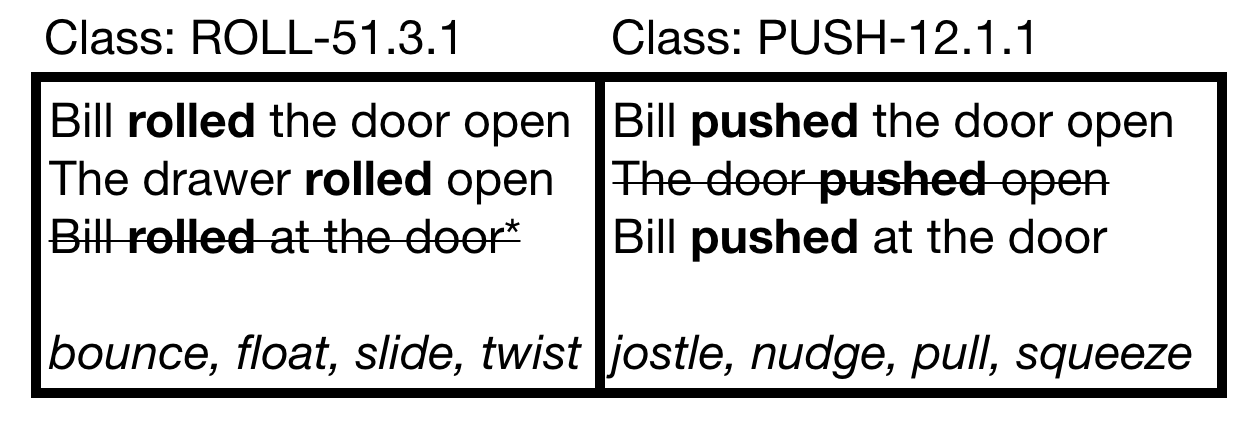
\includegraphics[width=0.5\textwidth]{VerbTable.png}
	\caption{\label{fig:frog} Two verb classes from VerbNet (Palmer, CITATION), showing a subset of frames that are used to identify the classes, and examples of verb in that class.)}
\end{figure}

No semantic criteria are used to generate the classes, but the verbs nevertheless share aspects of meaning.  *Note that this sentence is ungrammatical in the \emph{conative reading} (Bill attempted to roll the door but didn't move it, in parallel with "Bill pushed at the door.") The only grammatical interpretation is the \emph{locative reading} where Bill himself rolls towards the door. 
\cite{10.2307/41217861}
Levin (1993) developed the notion of a verb class. This classification was extended and enriched by Verbnet, a database of about 8000 verb/class instances. The website of VerbNet describes a verb class:

\begin{displayquote}
	“Each verb class in VN is completely described by thematic roles, selectional restrictions on the arguments, and frames consisting of a syntactic description and semantic predicates with a temporal function, in a manner similar to the event decomposition of Moens and Steedman (1988).”
\end{displayquote}

We are interested in demonstrating that GLoVe encodes syntax information; thus, the most natural thing to try and predict are the frames a verb fits into. It is worth noting that in VerbNet, whether or not a verb fits in a frame is true or false, with no gray area - in practice, such judgments by humans are much fuzzier. 


Any verb in VerbNet belongs to some number of classes, and each class expresses some number of the 291 frames. Suppose we number the frames $f_1... f_{291}$. The notion of a “binary frame vector” associated to a verb is as follows: Suppose a verb vhas associated binary frame vector $v$, then we say 
$v_i =1$ if $v$ belongs to frame $i$ in any of its class instantiations, and 0 otherwise.

\subsection{Distributional models of verb semantics}

IDAN/KYLE WRITE - can be short, focus on what's different about this - primarily, we treat verbs just like any other words. Describe/cite what Glove is. This is the section to head off objections about sense/POS disambiguation as well - say whether we're using a Glove version that does, acknowledge any limitation, and move on. )

\cite{pennington2014glove} presented informationally rich word embeddings that performed well on analogy tasks and similarity tasks. 

On the other hand, for most of the verbs in VerbNet, we have GLoVe vectors. For this project, I wanted to make use of distributional information from Wikipedia and Twitter - thus, GLoVe vectors from both were concatenated to form a 400-dimensional vector of real numbers that encodes its distributional information. 

\section{Predicting VerbNet frames from GLoVe, and vice versa}

\subsection{Summary of the prediction task - VerbNet from GLoVe}

We can reduce from the problem of recovering verb syntax from GLoVe to learning a good approximate mapping from the 400-dimensional to the 291-dimensional space of binary frame vectors. In the field of machine learning, this is known as a multi-label classification problem.

We’ll randomly shuffle the set of verbs for which we have both GLoVe vectors and frame vectors into a training set of 2949 verbs, and a validation set of 737 verbs, i.e. the standard 80/20 training/validation split for most machine learning problems. By learning a mapping from glove vectors to frames on the training data and checking its precision (see part 2) on the validation data, we will attempt to demonstrate that we can in fact successfully recover syntax information from GLoVe.

One of the simplest possible models was chosen for classification: a logistic regression model. Since a logistic regression model is a binary classifier, and we are interested in 291 classification problems, we simply concatenate and separately train 291 independent logistic classifiers to predict the frame vector of a verb from its GLoVe vector.

An advantage of a logistic regression model is that its transparency will allow us to directly examine the weights on each dimension of GLoVe - in short, it may be able to find which dimensions of GLoVe are most diagnostic, for syntax purposes.

To ensure robust predictions, positive training examples in both training and testing sets, and to simplify the problem of disentangling the data into training and testing sets such that this latter condition is satisfied, all frames with 5 or fewer positive training examples have been excluded from our prediction task. Since there are 232 frames with more than 5 positive training examples, we restrict our investigation to these frames (for the time being).

\subsubsection{Discussion of Results}

Since we are evaluating hundreds of independent binary classifiers, the Area Under the Receiver Operating Curve (AUROC) seems a fair benchmark for our model. The receiver operating curve of a binary classifier is essentially the true positive rate of the classifier, plotted against its false positive rate. That is, the probability it will correctly classify a positive example as a function of the probability it will incorrectly classify a negative example. When these points are joined they form a curve, and the area under it, or AUROC, measures the effectiveness of a binary classifier by giving a number between .5 and 1.0 that measures the strength of the tradeoff between false positives and true positives - at .5, a model is no better than a random classifier. At 1.0, the model classifies all training examples perfectly. 

After fitting the 232 logistic regressions on the training data, we now consider their performance on the testing data. We can plot the receiver operating curves atop one another as below. They appear vary widely, but there is no mistaking that the average predictive strength is well above a random classifier. However, some spuriously trained models do quite poorly - take a look at the curves that fall below the random classifier benchmark line $y = x$.  

\begin{figure}
	\centering
	\includegraphics[width=0.5\textwidth]{AUC_plot5.png}
	\caption{\label{fig:frog} 232 frames with minimum 5 training examples, AUC average = .8431}
\end{figure}

It is easy to see that, on average, predicting frames from GLoVe vectors using a logistic regression classifier does better than random chance. But there is a lot of variance in how good the model is for different frames. Let's see what happens when we raise the threshold for training examples.

\begin{figure}
	\centering
	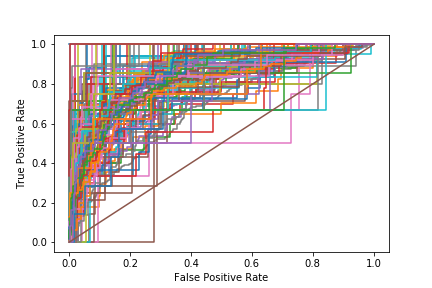
\includegraphics[width=0.5\textwidth]{auc_plot15.png}
	\caption{\label{fig:frog} 155 frames with minimum 15 training examples, AUC average = .8421}
\end{figure}

\begin{figure}
	\centering
	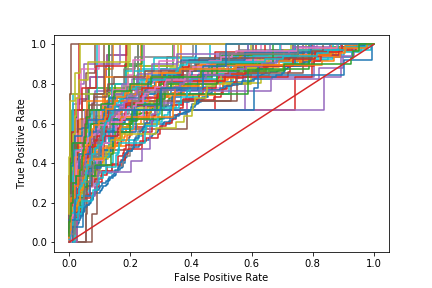
\includegraphics[width=0.5\textwidth]{auc_plot30.png}
	\caption{\label{fig:frog} 93 frames with minimum 30 training examples, AUC average = .8409}
\end{figure}

\begin{figure}
	\centering
	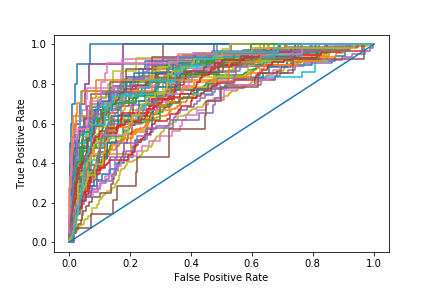
\includegraphics[width=0.5\textwidth]{auc_plot50.png}
	\caption{\label{fig:frog} 60 frames with minimum 50 training examples, AUC average = .8111}
\end{figure}

It's clear from the above plots that model stability and performance goes up as a function of the number of training examples. What's encouraging is that AUC seems to stabilize as well. Let's take a look at a scatterplot of AUC against the number of training examples.

\begin{figure}
	\centering
	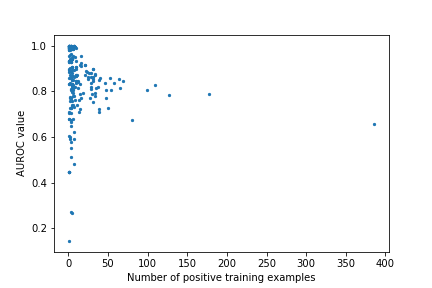
\includegraphics[width=0.5\textwidth]{auc_scatter5.png}
	\caption{\label{fig:frog} }
\end{figure}

As training examples (the X-axis) increases, the spread in AUC tends to decrease, all the while stabilizing at around .75, confirming our hypothesis.

It seems clear that our model is predicting syntax reasonably well from GLoVe vectors. How can we be sure we have not overfitted a model? For one, the training data was thrown away after model fitting, and all the results you see above are on the test set. This alone is reason to believe we have not overfitted to our data.

Suppose we scrambled the assignment of verbs to frames. Our model could still pick up on the distributional information of frames (e.g. this frame occurs 30\% of the time, so with a false positive tolerance of 70\% or more we should predict it always), but the GLoVe vector observations for a verb would be meaningless. How does such a model do? Let us examine their collective ROC plots in figure 7.

\begin{figure}
	\centering
	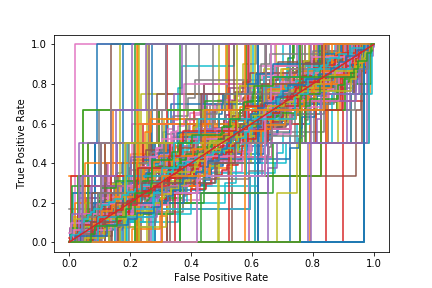
\includegraphics[width=0.5\textwidth]{auc_plot5rand.png}
	\caption{\label{fig:frog} }
\end{figure}

\begin{figure}
	\centering
	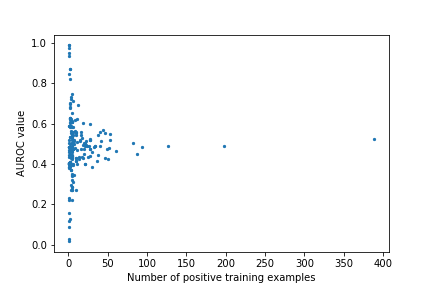
\includegraphics[width=0.5\textwidth]{auc_scatter5rand.png}
	\caption{\label{fig:frog} }
\end{figure}

These models perform no better than random chance. Indeed, it's clear from figure 8 that in this case that 
\[  \lim_{\# \text{training examples} \rightarrow \infty} AUROC = .5 \]
Which is as we expect for a collection of fundamentally random (uninformed) classifiers. This is good because it tells us GLoVe vectors give us frame information when (and only when) this information is correctly paired, which is another confirmation of our hypothesis.

\subsection{Dimensionality reduction of word embeddings}
It is possible to make predictions from our word embeddings that are nearly as good using only a fraction of the dimensionality. Given data which we have split into 80\% training and 20\% testing, we can use the training data to discover a transformation designed to preserve syntax information, that maps our word embeddings from $\mathbb{R}^{100}$ to $\mathbb{R}^d$ where $d < 100$ (details in appendix). We can then re-train our logistic regressions on the reduced-dimension training data and explore their performance on the reduced-dimension test set. 

Suppose we restrict to the 183 frames most represented in our set of verbs, and ask how performance of our frame classifiers degrades as a function of the number of original dimensions of our word embeddings that we use. Consider figure 9, a plot of the average AUROC over the 183 frame classifers as a function of the number of dimensions onto which we have projected our word embeddings.

\begin{figure}
	\centering
	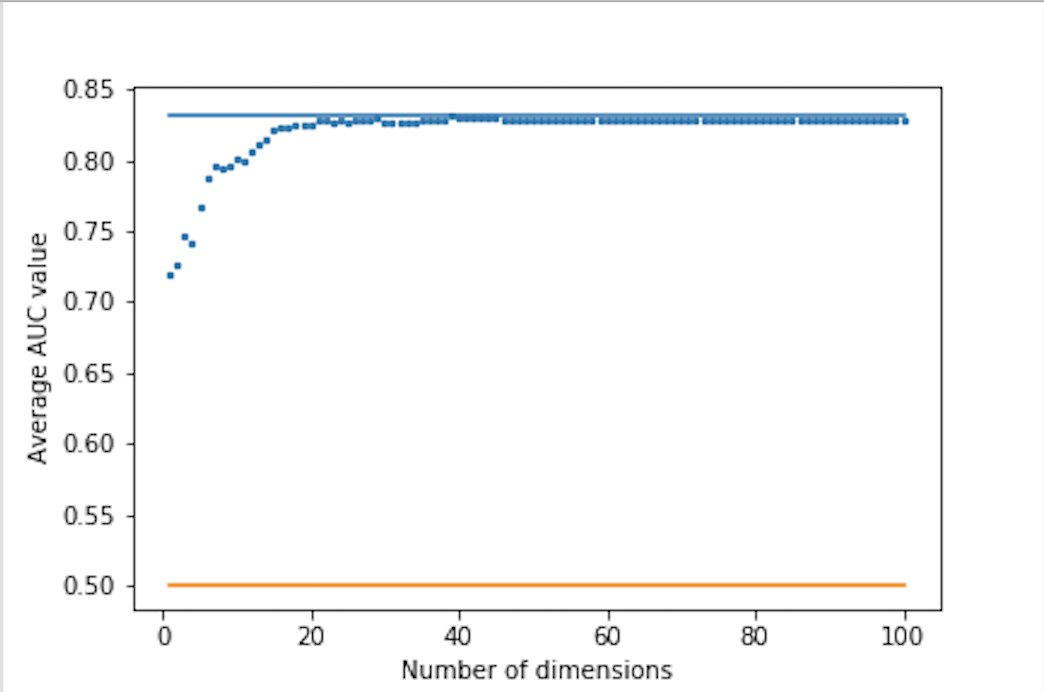
\includegraphics[width=0.5\textwidth]{aucbydimension.png}
	\caption{\label{fig:frog} Orange line is performance of the baseline random predictor, blue line is predictor trained on full-dimensional GLoVe data}
\end{figure}

 
\section{Modeling human similarity judgments from VerbNet and GLoVe}

\section*{Acknowledgments}

The acknowledgments should go immediately before the references.  Do
not number the acknowledgments section. Do not include this section
when submitting your paper for review.

% include your own bib file like this:
%\bibliographystyle{acl}
%\bibliography{acl2017}
\bibliography{acl2017}
\bibliographystyle{acl_natbib}

\appendix

\section{Appendix}
\label{sec:supplemental}
In this section we describe our method of reverse-PCA for discovering syntactically diagnostic axes of the space of word embeddings.

Consider our prediction task: recall that we are predicting $L$ frame labels from an input space of dimension $D=100$. For a single label, logistic regression over our data of word embeddings is formulated such that, given $n$ input data $\{\vec x\}_{i=1}^n \in \mathbb{R}^{100}$ and corresponding labels $\{\vec y_i\}_{i=1}^n \in \{0,1\}$, we learn a weight vector $\beta_1$ and bias $\beta_0$ that gives optimal prediction probabilities
\[ P(\vec x_i \text{ is labeled } 1) = (1 + e^{-(\beta_0 + \vec x_i \cdot \beta_1)})^{-1} \]
In other words, it is easy to see that we predict $\vec x_i$ to have label 1 if 
\[  \beta_0 + \beta_1^T x_i > 0 \]
And we predict label 0 otherwise, because the probability will be less than $\frac{1}{2}$. But the takeaway here is that each frame has a weight vector $\beta_1$ on the space of word embeddings that measures, inuitively, how important each dimension is.  

Suppose we ran PCA on the space of weight vectors $\beta_1^i$, where the number of data points is precisely the number of frames $i$, $i \in \{1...L\}$. Mathematically, this gives an orthonormal transformation $U$ such that for any weight vector $\beta_1^i$, 
\[ \beta_1 \approx U^T(U(\beta_1 - \mu)) + \mu \] 
Where $\mu$ is the mean of the data $\{\beta_1^i\}_{i=1}^L$. Notice that intuitively, this means
\begin{align*} 
P(\vec x_i \text{ is labeled } 1) &= (1 + e^{-(\beta_0 + \vec x_i \cdot \beta_1)})^{-1}  \\
&\approx (1 + e^{-z})^{-1} 
\end{align*}
Where we have defined
\[ z := \beta_0 + \vec x_i \cdot (U^T(U(\beta_1 - \mu)) + \mu) \]
Simply regrouping parentheses, we obtain
\[ z := \beta_0 + (\vec x_i  U^T)(U(\beta_1 - \mu)) + \mu) \]
The key fact is that is a linear function of $\vec x_i U^T$, which is in fact a reduced-dimension representation of $\vec x_i$. Moreover, this linear function will be implicitly learned via a logistic regression if we transform our input data $\vec x_i$ by left-multiplication of $U^T$, and since our choice of $U$ was to minimize reconstruction loss on the weight vectors $\beta_1$, we should be able to get prediction accuracy close to that of when we used our original data set. 

As in the previous section, we split our data into 80\% training and 20\% testing. The difference here is that we first train a logistic regression to learn the weights $\beta_1$ from our training set, and then recover the transformation $U^T \in \mathbb{R}^{100 \times n}$ by running PCA on those weights. Then we transform our training AND testing data by left-multiplication of $U^T$, and train another logistic regression with the transformed data and the same labels. 

\end{document}
